%##########################  CHAPER 6: APPLICATION  #######################

\chapter{Entwicklung der Anwendung}\label{kap:application}

Dieses Kapitel beschreibt die Realisierung der Anwendung 
als autonomes Kamera System zur, 
Wildtiererkennung, welches auf einem Raspberry Pi 4 läuft.

Dabei wird es neben der Implementierung der Inferenz für eines der 
traininierten Modelle, auch um die Auswahl einer 
nachtsichtgeeigneten Kamera und der implementierung 
einer Kommunikationsmöglichkeit zur übermittlung 
der Daten gehen.



%-------------------------  SECTION 1: AUFBAU  ------------------------
\section{Hardware}\label{sec:aufbau}


Der Aufbau der Anwendung besteht aus einem Raspberry Pi 4, auf dem 
der Programmcode läuft, sowie dem Neural Compute Stick 2
für die Inferenz, welcher über eine USB Schnittstelle
mit dem Raspberry Pi verbunden wird.

Zur aufnahme der Bilder wurde ein Raspberry Pi Kamera Modul mit 
5MP OV5647 Sensor der Marke Longrunner verwendet.
Dieses ermöglicht durch mechanisches zu und abschalten eines Infrarot 
Filters vor die Linse zwischen Tag und Nachtsicht zu wechseln.
Der dafür verwendete Magnetschalter wird dabei über einen 
Helligkeitsensor getriggert.
Im Infrarotmodus befindet sich der Filter nicht 
vor der Linse, wodurch neben den elektromagnetischen 
Wellen des Sichtbaren Lichts auch die etwas langwelligeren 
(850nm) des Infrarot Spektrums auf die Linse treffen und 
verarbeitet werden können.

Zudem verfügt die Kamera über zwei Infrarot LEDs, 
sodass auch Aufnahmen bis zu 3m Entfernung
in völliger Dunkelheit gemacht werden können. Diese haben 
den vorteil gegenüber normalen Scheinwerfern, 
das die Tiere von keiner Sichtbaren Lichtquelle 
gestört oder verscheucht werden.
verbunden wird das Kamera Modul über die CSI 
(Camera Serial Interface) 
Schnittstelle des Raspberry Pi's.
\vspace{1cm}



%https://www.amazon.de/gp/product/B07R4JH2ZV/ref=ppx_yo_dt_b_asin_title_o01_s00?ie=UTF8&psc=1


\begin{minipage}{0.55\textwidth}
    \centering
    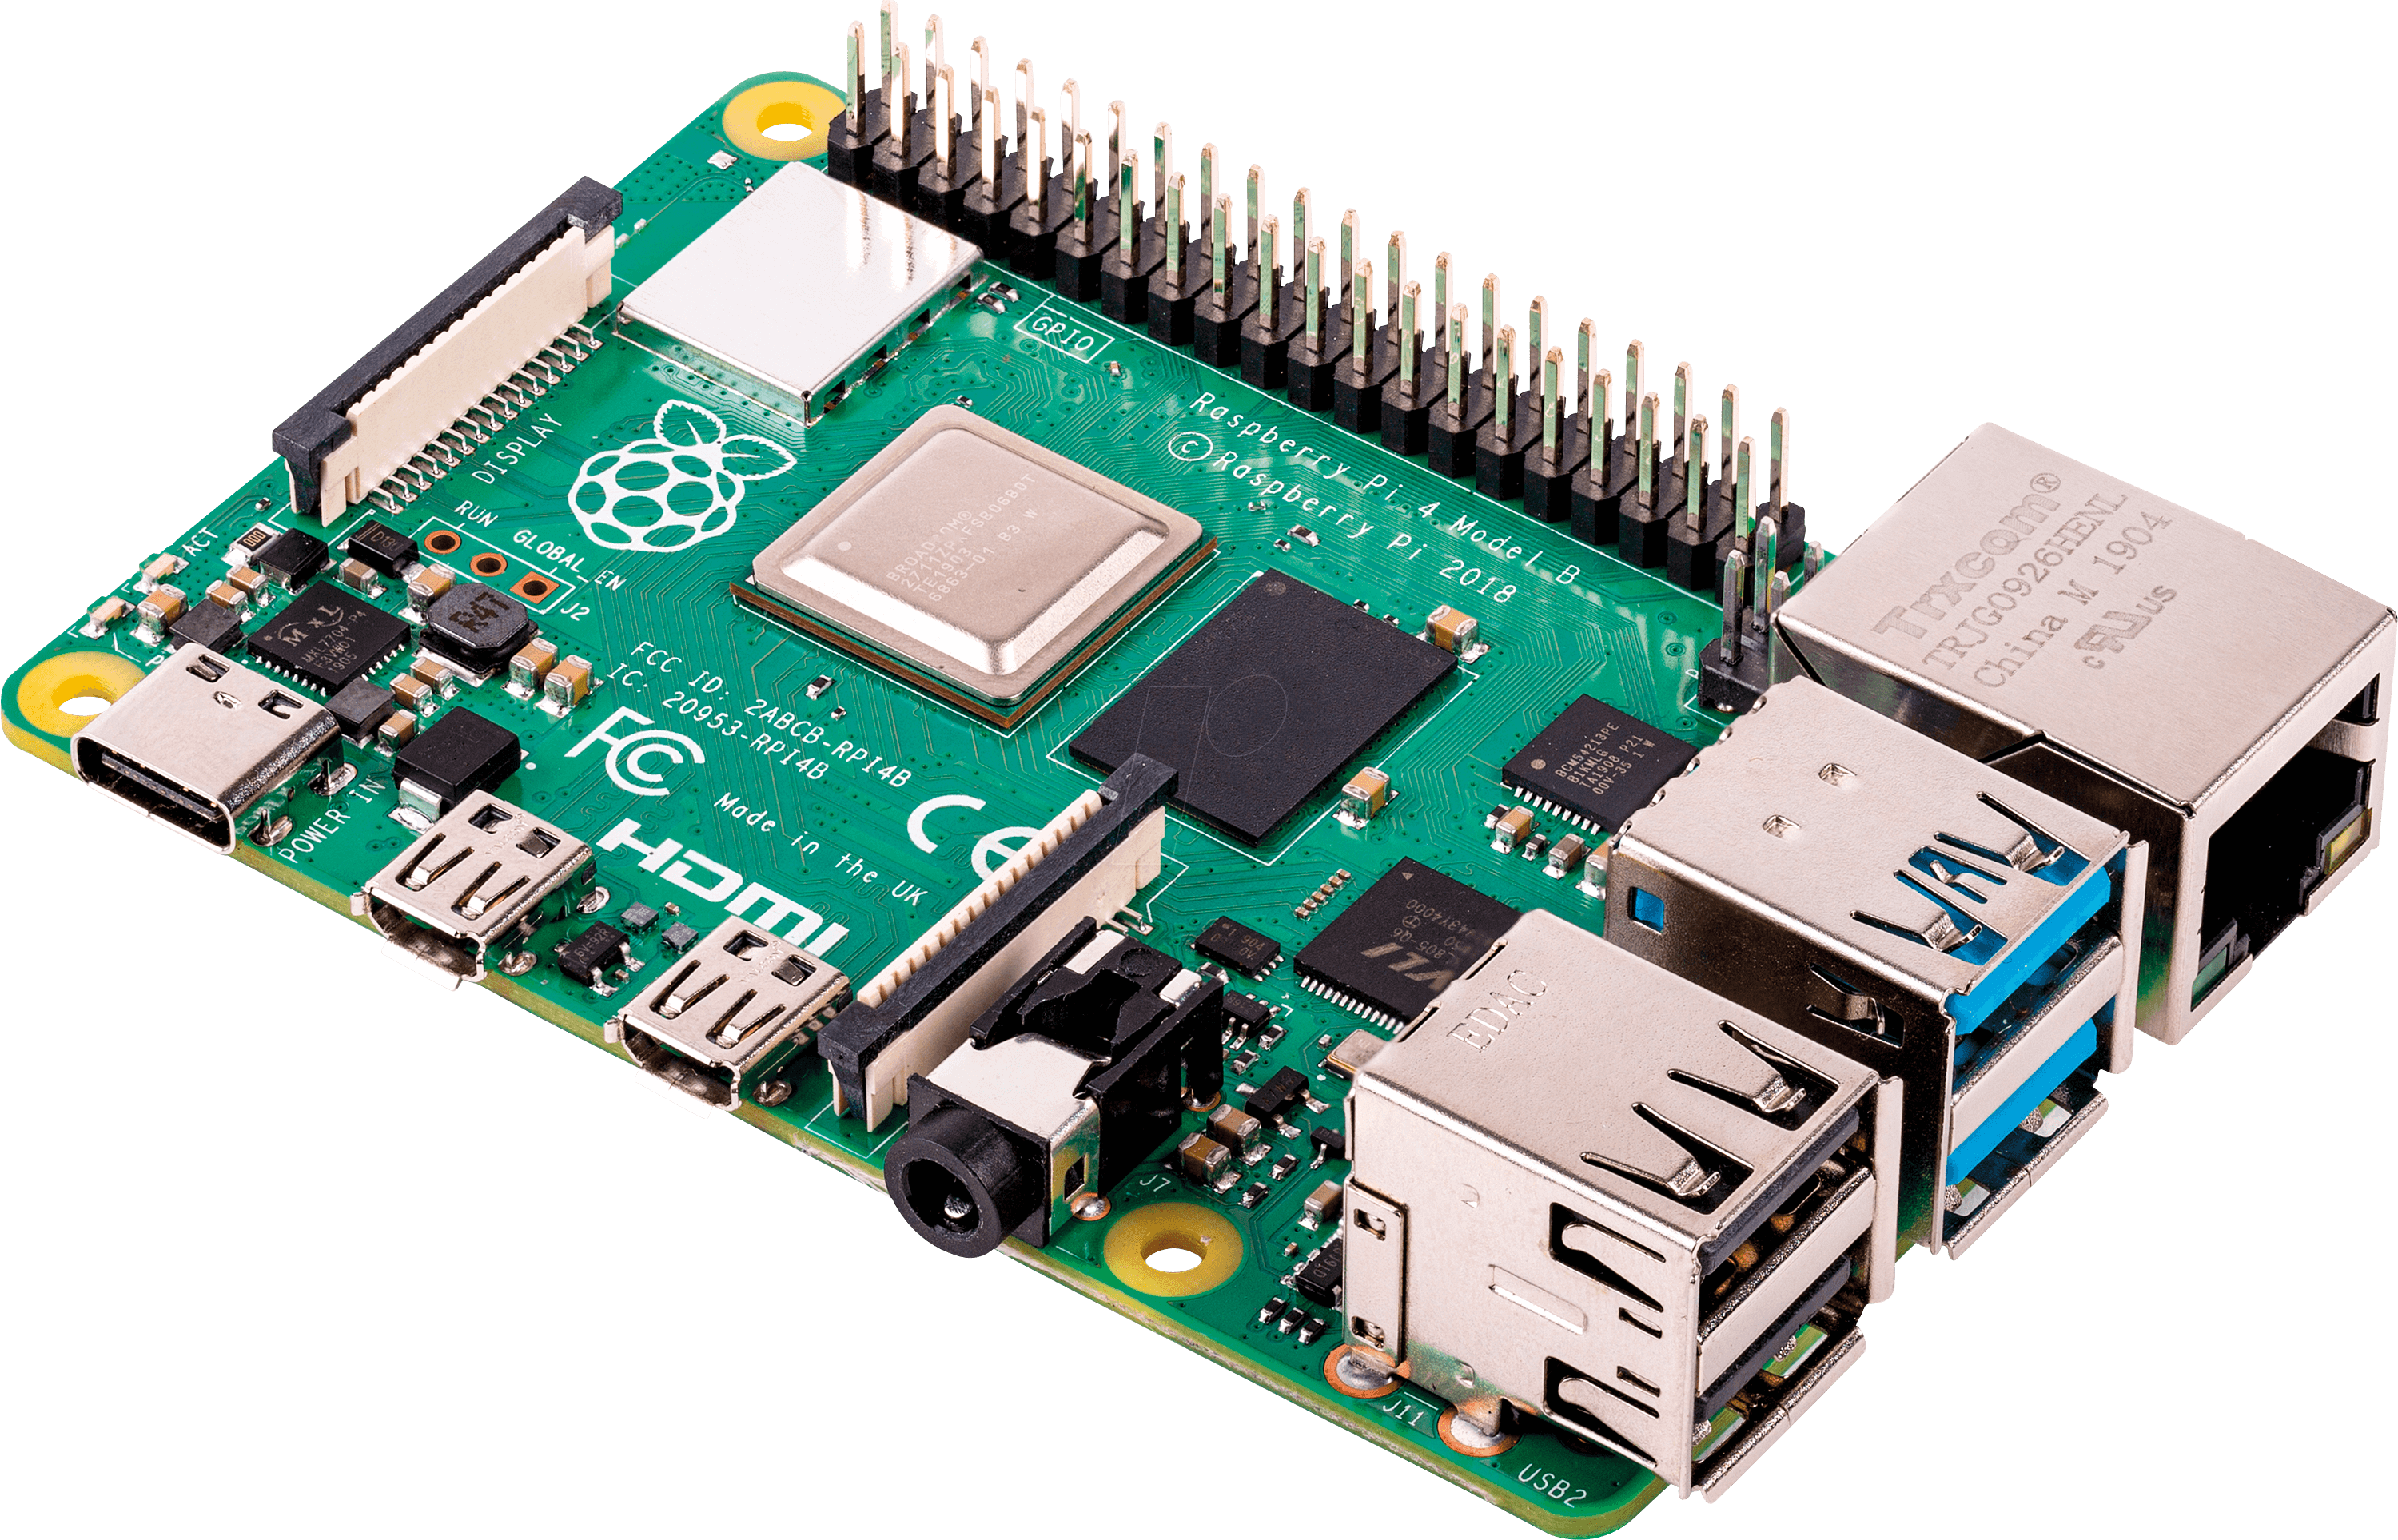
\includegraphics[width=0.8\textwidth]{./Bilder/raspberrypi_4.png}
    \captionof{figure}{Raspberry Pi 4}
    \label{img:raspberrypi}
\end{minipage}
\begin{minipage}{0.45\textwidth}
    \centering
    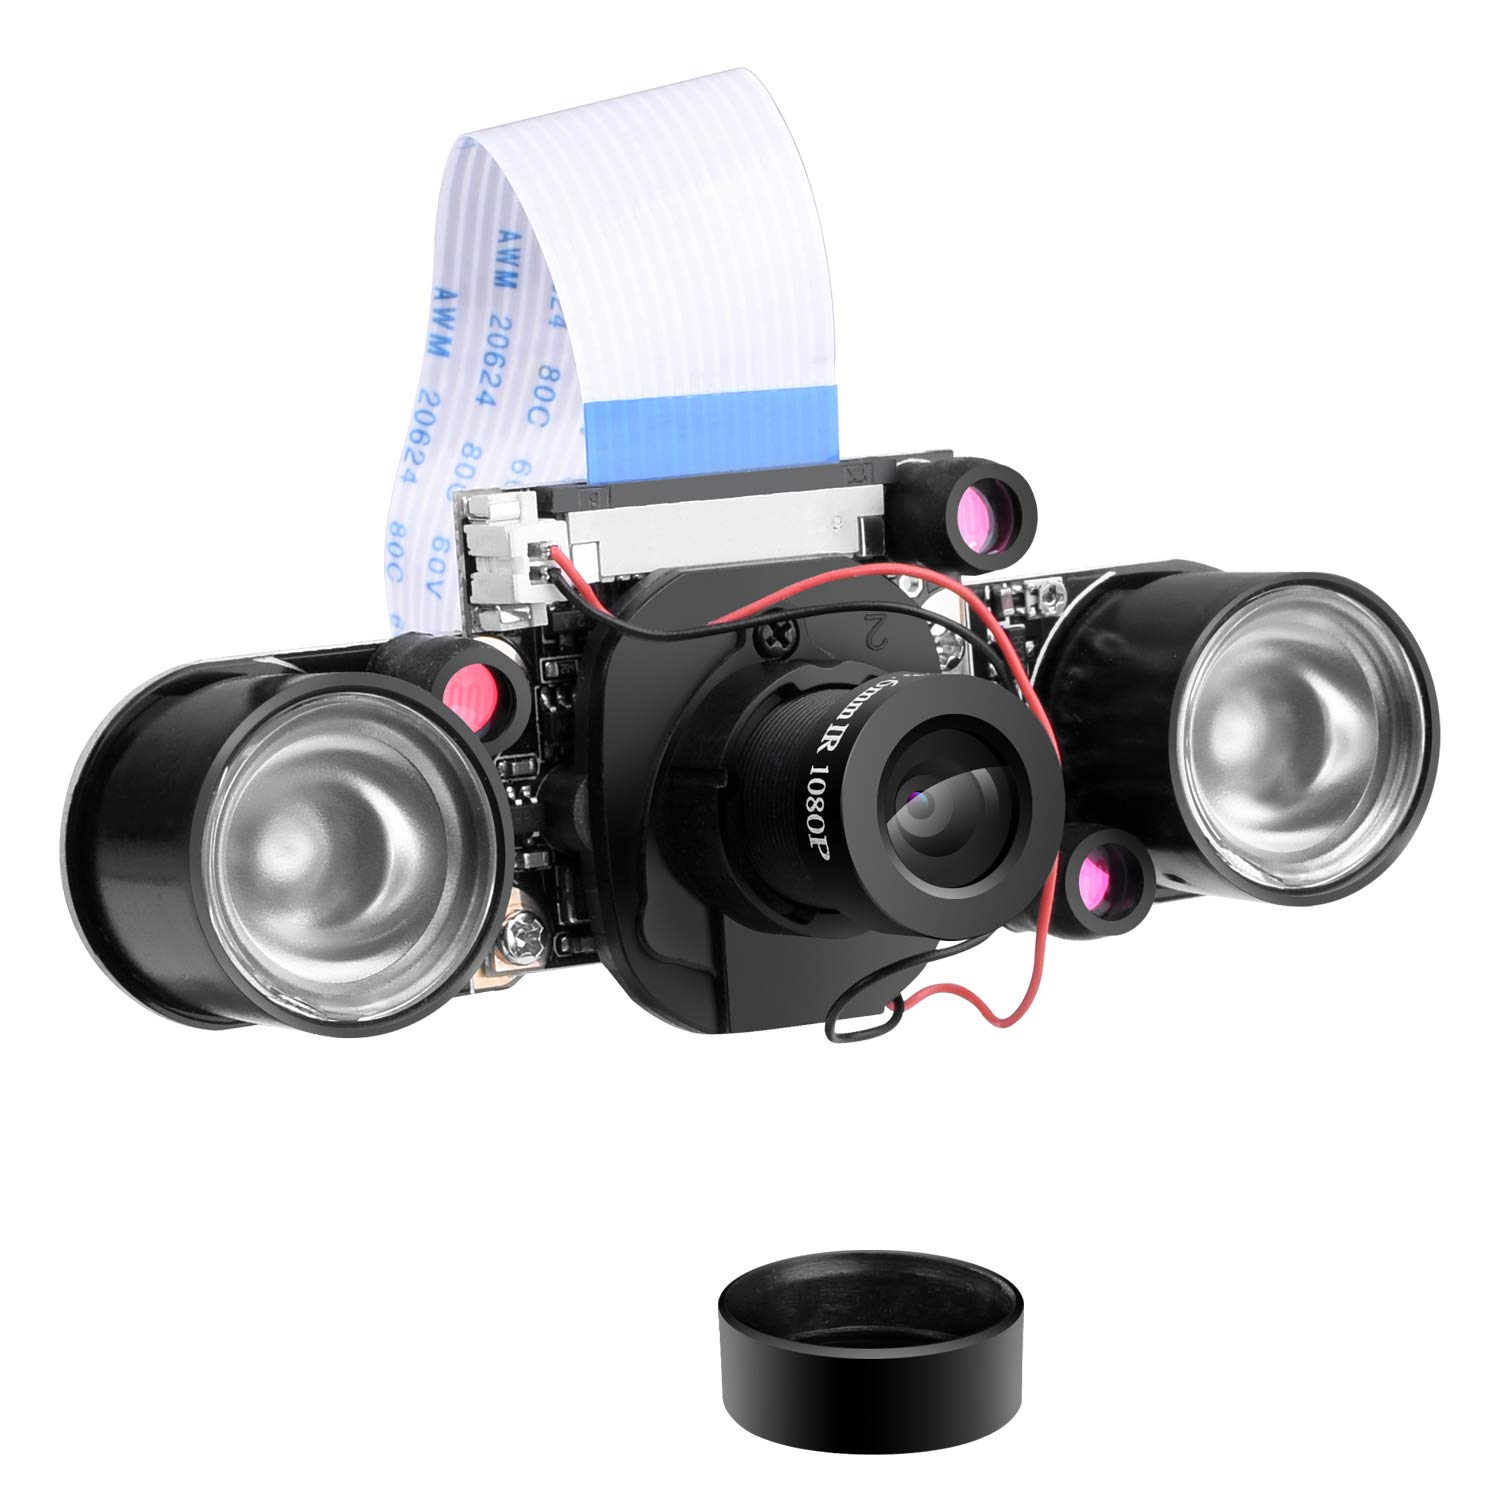
\includegraphics[width=0.8\textwidth]{longrunner.jpg}
    \captionof{figure}{Longruner Kamera Modul}
    \label{fig:rpicam}
\end{minipage}
\vspace{1cm}


Desweiteren wurde für eine mobile Internetverbindung 
der \textit{Huawei E3531 SurfStick} und zu Stromversorgnung
eine Powerbank verwendet.



% https://www.amazon.de/gp/product/B00HSZEY34/ref=ppx_yo_dt_b_asin_title_o00_s00?ie=UTF8&psc=1


\section{Software}


Die Implementierung der Anwendung für den Raspberry Pi wurde in Python.
vorgenommen. 
Dabei sind die Funktionalitäten zur Objekerkennung in einem Script 
\textit{detection.py} 
und die für die Verbindung und Senden der Daten in einem 
\textit{connection.py} Script aufgeteilt.

Der Kamera Inputstream ist in einem \textit{main.py} Script implementiert, 
von dem aus auch die in Abbildung \ref{fig:class_diagram} 
dargestellten Klassen, welche in \textit{detection.py}
und \textit{connection.py} definiert sind verwendet werden.


\vspace{1cm}
\begin{minipage}{0.75\textwidth}
    \centering
    \underline{detection.py}
\end{minipage}
\begin{minipage}{0.25\textwidth}
    \centering
    \underline{connection.py}
\end{minipage}
\begin{figure}[H]
    \centering
    \begin{tikzpicture} 

    
    
            \umlclass{Motion}{ 
              statickBackground : np.array
              }{ 
              + detectMotion() : bool \\
              + resetBackground() : void
            }
        
            \umlclass[y=-4]{InferenceModel}{ 
                string : plugin
                strin : device
                }{ 
                + createExecInferModel() : ExecInferModel
              }
        
            \umlclass[y=-2, x=6]{ExecInferModel}{ 
                shape : ioBlob\\
                detected : array
                }{ 
                + inferFrames() : status \\
                \# status[0] num infered\\
                \# status[1] num detected\\
                \# status[2] num saved\\
                - save() : void
                }
        
    
        \umlclass[x=11, y=-2]{Connection}{ 
            string logindata
            }{ 
            + login() : bool \\
            + connect() : server, port\\
            + send() : bool\\
            + disconnect() : bool\\
            + sendEmail(email, text) : boiol
          }

    
    \end{tikzpicture}
            
    \caption{Klassendiagramm}
    \label{fig:class_diagram}
\end{figure}
\vspace{1cm}


\textit{Motion} ist eine Klasse zur Erkennung von Bewegung im Kamera 
Input Stream, \textit{InferenceModel} und \textit{ExecInferModel} 
dienen der Inferenz und \textit{Connection} dem Aufbau einer
Verbindung zu einem Pc sowie dem Senden der Daten über diese Verbindung.

Durch geeigneten Implementierung des Applikationsablaufes,
sollte eine Möglichkeit gefunden werden, trotz langsamer Inferenzzeiz,
mit dem Faster R-CNN alle relevanten Frames, 
also die in denen Tiere zu vermuten sind, inferieren zu können.
Dafür wurde die Annahme gemacht, dass zur Laufzeit der 
Anwendung nicht durchgehend inferiert werden muss,
sich also Zeitweise keine Tiere und damit auch keine 
Bewegung vor der Kamera befinden.

Um Bewegungen feststellen zu können, 
wurde, mithilfe der Library OpenCV ein Bewegungsmelder 
implementiert.
Dieser speichert zu begin des Kamera Streams ein Referenz
Frame ab, mit dem alle weiteren Frames verglichen werden.
Beträgt der Abstand einzelnen Pixelwerte im 
Graustufenbereich mehr als ein bestimmter 
Threshhold, wurde eine Bewegung erkannt.
Indem nun die Frames, welche der Kamera Stream permanent 
liefert, zunächst auf Bewegung überprüft wurden, 
ließ sich unnötiges inferieren, was Zeit und 
und Leistung kostet, vermeiden.
Frames die bewegung enthalten und aufgrund der langsameren 
inferenzzeit des Faster R-CNN nicht sofort inferiert 
werden können, werden in einem Buffer zwischen 
gespeichert und in Phasen zu denen keine Bewegung stattfindet 
inferiert.

Dafür musste der im Abschnitt \ref{sec:infertime} beschriebene
Asynchrone Inferenz Ablauf dahingehend angepasst werdem, dass 
keine Blockieren mehr stattfindet, diese also komplett 
zeitasynchron zu den Input Frames ablaufen kann.
Der Gesamtablauf der Applikation ist in Abbildung 
\ref{fig:flowchart_appl} 
schematisch als Flussdiagram dargestellt.



\vspace{1cm}
\begin{figure}[H]
    \centering
    \tikzset{
    desicion/.style={
        diamond,
        draw,
        text width=4em,
        text badly centered,
        inner sep=0pt
    },
    block/.style={
        rectangle,
        draw,
        text width=10em,
        text centered,
        rounded corners
    },
    arrow/.style={
        draw,
        >=latex,
        ->
    }
}


\begin{tikzpicture}
    \node (A) [desicion] {entschei\\dung};
    \node (B) [block, below of=A, node distance=3cm, text width=5em] {bock};
    \node (C) [block, right of=A, node distance=0.5\textwidth] {noch ein\\bock};


    \draw[arrow] (A) --  node [left, fill=white!30] {yes} (B);
    \draw[arrow] (A) -- node [below, near end] {crap} (C); 
    \draw[arrow] (B) -| node [near start, fill=white] {yes} (C);

\end{tikzpicture}
    
    \caption{Main Applikation}
    \label{fig:flowchart_appl}
\end{figure}
\vspace{1cm}

Wird in inferierten Frames mehrfach nichts 
erkannt, wird das referenz Frame des 
Bewegungsmelders neu gesetzt, 
da vermutlich sich das Hintergrundbild 
geändert hat.

Erkannte Objekt werden in einem Dictionary zusammen 
mit Klassenname (cls), Wahrscheinlichkeit(p)
Anzahl an Erkennungen (N) sowie die Bounding 
Box Koordinaten (Roi, Region of Interest) 
abgespeichert.

Nach 10 Erkennungen des selben Objekts, wird dieses 
als lokale Bilddatei abgespeichert und ein 
Send-Requst an die Main zurückgegeben.

Diese prüft ob eine Verbindung zu einem 
anderen Gerät besteht, stellt diese gegebenenfalls her 
und sendet die Bilder.

Um nicht permanent die Verbindung zu einem Pc aufrecht erhalten 
zu müssen, was das Datenvolumen des mobilen Internets, des 
Raspberry schneller aufbrauchen würde, wird diese nach einer 
bestimmte zeit ohne Bewegung getrennt.


\subsection*{Inferenz}

Der in Abschnitt \ref{sec:infertime} beschriebene asynchronen
Inferenzablauf wurde dahingehend angepasst, dass eine beliebige Anzahl 
an Inferenz Requests verwendet werden können 
und dass das Warten auf ein Inferenz Ergebnis
nicht mehr blockierend ist.
Dafür wurde der Timeot in der Wait Funktion auf 
$0ms$ gesetzt.
Durch vorheriges abspeichern der jeweiligen zu 
inferierenden Frames, kann eine richtige zuordnung 
der Inferenz Ergebnisse zu den Frames erfolgen.
Der Pseudocode in Algorithmus \ref{code:infer_async_neu} stellt
grob den Inferenzablauf dar.

\begin{algorithm}[H]
    \caption{Asynchrone Inferenz, ohne Blockierung}
    \label{code:infer_async_neu}
    \begin{algorithmic}
    \WHILE{\TRUE}
    \STATE capture FRAMES
        \FOR{all InferRequests}
            %\STATE Status $\leftarrow$ \textbf{wait} for InferRequest
            \IF {\textbf{wait} for InferRequest == 0}
                \STATE Result $\leftarrow$ InferRequest.output
            \ENDIF
            \IF {Buffer \textbf{not} empty}
                \STATE preprocess InferRequest
                \STATE \textbf{start} InferRequest
            \ENDIF
            \IF{Result not NULL}
                \STATE process Result
            \ENDIF
        \ENDFOR
    \ENDWHILE
    \end{algorithmic}
\end{algorithm}    





\subsection*{Connection}

Um die Bilder mit erkannten Tieren an ein anderes Gerät 
z.B. einen Pc senden zu können, musste eine Verbindung
hergestellt werden, die auch über verschiedene Netzwerke 
hinweg funktioniert.

Um unabhängig von Router Konfigurationen des Heimnetzes zu sein, 
wurde mithilfe des Dienstes \textit{remot3.it} \cite{remoteit}
eine Cloudbasierte Remote Verbindung hergestellt.
Mit dieser war es möglich eine Proxy SSH Verbindung, 
über das Internet herzustellen, ohne von einer Firewall 
blockiert zu werden.


\begin{figure}[H]
    \centering
    \def\svgwidth{0.7\textwidth}
    \input{Bilder/diagram-connect.pdf_tex}
    \caption{Prinzip Proxy Verbindung}
    \label{fig:remoteit}
\end{figure}

Da die Daten vom Raspberry Pi aus automatisiert gesendet 
werden sollten, wurde der Pc als Remote Gerät implementiert.
Gesendet wurden die Daten über das Secure Copy Protocol welches 
das hergestellte Secure Shell Protocol (SSH) verwendet.
Dieses lässt sich über folgendes Kommando,
welches im \textit{connectin.py}
Script ausgeführt wird verwenden:
\begin{itemize}
    \item[\texttt{\$}] \texttt{scp -P port file.jpg user@proxyserver /zielpfad/file.jpg}
\end{itemize}

Server und Port werden dabei von remoteit generiert, \textit{file.jpg}
ist das zu sendende Bilde und \textit{user} der Nutzername des Geräts,
an welches gesendet wird.
Um das Einloggen sowie den Verbindungsauf- und Abbau 
über remote.it zu einem Gerät zu automatisieren
bietet remote.it eine API mit der über Post- und Get-Requests
die Befehle dafür programmatisch aufgerufen werden können.




 









% \input{Bilder/class_diagramm/class_diagramm.latex}

% \begin{minipage}{0.3\textwidth}
%     \centering
%     \input{Bilder/diagramme/class_detection.tex}    
% \end{minipage}
% \begin{minipage}{0.3\textwidth}
%     \centering
%     \input{Bilder/diagramme/class_connection.tex}
% \end{minipage}
% \begin{minipage}{0.3\textwidth}
%     \centering
%     \input{Bilder/diagramme/class_motion.tex}
% \end{minipage}

% oder

%\input{Bilder/diagramme/detection_package.tex}

% oder 





%Asynchrone inferenz
%https://docs.openvinotoolkit.org/latest/_demos_python_demos_object_detection_demo_ssd_async_README.html

% main
% \begin{algorithm}[H]
%     \caption{Main Program}
%     \begin{algorithmic}

%     %\STATE INIT EXEC_NET, CAM

%     \WHILE{\TRUE}
%         \STATE capture frame
        
%         \IF{frame has motion}
%             \STATE $buffer \leftarrow frmae$
%         \ENDIF

%         \IF{buffer is empty}
%             \STATE disconnect
%         \ENDIF

%         \STATE result = inferFrames (buffer)

%         \FOR{all results}
%             \STATE process results
%             \IF {saved}
%                 \STATE sendRequest = \TRUE
%             \ENDIF
        

%             \IF {no detectoin for 20 times}
%                 \STATE reset motion background
%                 \STATE delete buffer
%                 \IF {connected}
%                     \STATE disconnect
%                 \ENDIF
%             \ENDIF

%         \ENDFOR

%         \IF {send all every minute}
%             \STATE save current detections
%             \STATE sendRequest = \TRUE
%         \ENDIF

%         \IF{sendRequest == \TRUE}
%             \IF{not logged in}
%                 \STATE log in
%             \ENDIF

%             \IF{not connected}
%                 \STATE connect
%             \ENDIF

%             \STATE server, port $\leftarrow$ connection

%             \STATE sendRequest = \FALSE
%             \FOR{all saved images}
%                 \IF{send image $\rightarrow$ server, port}
%                     \STATE delete image
%                 \ELSE
%                     \STATE sendRequest = \TRUE
%                 \ENDIF
%             \ENDFOR

%         \ENDIF
%     \ENDWHILE


%     \end{algorithmic}
% \end{algorithm}



% \newpage

% \begin{center}
%     \rule{0.8\textwidth}{0.4pt}
%     \begin{lstlisting}[language=Python]
%         def infer_frames(Buffer, threshhold):
%             for idx, inferRequest in all inferRequests:
%                 status = inferRequest.wait(0) # nicht blockierend
%                 if status not ready:
%                     continue
                
%                 if idx in currentFrames:
%                     results = inferRequest.output
%                     frame = currentFrames[idx]

%                 if Buffer not empty:
%                     currentFrames[idx] = Buffer.pop()
%                     infer_frame = preprocess(currentFrames[idx])
%                     inferRequest.async_infer(infer_frame)

%                 if results or frame is None:
%                     continue

%                 for obj in all results:
%                     Class, Roi, Proba <- obj
%                     if Proba < threshhold:
%                         continue
                    
%                     coords <- Roi, frame.shape

%                     infered_frame = draw_rect(frame, coords)

%                     if proba > detectedObjects.proba
%                         replace detectedObjects

%                     if number of detections > x:
%                         send(frame)
                    
%     \end{lstlisting}
%     \rule{0.8\textwidth}{0.4pt}        
% \end{center}


% \centering\rule{0.6\textwidth}{0.4pt}
% \begin\centering{lstlisting}[language=Python]
%     def infer_frames():
%         for all requests:
%             do something \textbf{with} request

%             status = request.wait(0)
%             if status == done:
%                 res = requests.output
%                 frame = current[id]
% \end{lstlisting}
% \centering\rule{0.6\textwidth}{0.4pt}




% % inferenz
% \begin{algorithm}[H]
%     \caption{Asynchrone Inferenz}
%     \begin{algorithmic}
%     \WHILE{\TRUE}
%         \STATE capture Frame
%         \IF{Frame has Motion}
%             \STATE Buffer $\leftarrow$ Frame
%         \ENDIF
%         \FOR{$reqId$ = 0 to $reqMax$}
%             \IF {Model.reqests[$reqId$].wait(0)}
%                 \STATE result = Model.reqests[$reqId$].output
%                 \STATE inferedFrames $\leftarrow$ (result, currentFrames[$reqId$])
%                 \IF {Buffer not empty}
%                     \STATE currentFrames[$reqId$] $\leftarrow$ Buffer 
%                     \STATE inFrame = preprocess: currentFrames[$reqId$]
%                     \STATE Model.inferAsync($reqId$, inFrame)
%                 \ENDIF
%             \ENDIF
%         \ENDFOR
%         \RETURN inferedFrames
%     \ENDWHILE
%     \end{algorithmic}
% \end{algorithm}

% wobei die wait Funktion mit Timeout = 0 nicht blockierend ist.

% Dadurch war es möglich trotz langsamerer inferenz zeit als 
% capture zeit, durch zwischenspeichern alle frames zu inferieren, 
% unter der Annahme, das nur zeitweise bewegung erkannt und damit 
% inferiert werden muss.



